\documentclass[
  12pt,                     % Schriftgröße 12 pt
  a4paper,
  sfdefaults=false,
  toc=chapterentrywithdots,
  oneside,openright,
  titlepage,
  parskip=half,
  headings=normal,          % Reduziert die Größe der Überschriften
  listof=totoc,
  index=totoc,
  captions=tableheading,    % Bildunterschrift unter Tabellen
  listof=flat,
  final
]{scrbook}

% Schriftart Times New Roman
\usepackage{times}   


% details about your thesis
\newcommand{\titel}{Entwicklung eines VHDL-basierten Applikationsbeispiels zur Ablösung des FM350-2 Moduls durch das TM FAST Modul inklusive Integration in das TIA Portal und Aspekte des Software Engineerings}
\newcommand{\artderarbeit}{Bachelorarbeit}  % {Bachelorarbeit,Masterarbeit}
\newcommand{\autor}{Jan-Eric Gedicke}
\newcommand{\studiengang}{Informatik}  % {Informatik,Wirtschaftsinformatik,Medieninformatik}
\newcommand{\matrikelnr}{3643446}
\newcommand{\erstgutachter}{Prof. Dr. Trommler} %Prof.\,Dr.~Korbinian Riedhammer
\newcommand{\zweitgutachter}{Conrad, Maximilian} %Prof.\,Dr.~Bartosz von\,Rymon\,Lipinski
\newcommand{\betreuer}{} %M.Sc.\,~Martina Schmidt
\newcommand{\unternehmen}{Siemens}
\newcommand{\logo}{figures/TH-Nuernberg-RGB.png}
\newcommand{\keywords}{hot, fuzz}
 

% custom head and foot
\usepackage[automark]{scrlayer-scrpage}
\pagestyle{scrheadings}
\ihead{\headmark}
\chead{}
\ohead{\pagemark}
\renewcommand*\chaptermarkformat{\chapappifchapterprefix{\ }% 
  \thechapter.\enskip}

\RedeclareSectionCommand[tocindent=0pt]{section}
\RedeclareSectionCommand[tocindent=0pt]{subsection}
%\RedeclareSectionCommand[tocnumwidth=70pt]{chapter}

\usepackage{scrhack}

% other packages
\usepackage[utf8]{inputenc}
\usepackage[T1]{fontenc}
\usepackage{lmodern,relsize,textcomp,csquotes}
\usepackage{amsmath,amsfonts}
\usepackage[ngerman]{babel}  % flip for German thesis
\usepackage[final]{graphicx}
\usepackage{setspace,geometry,xcolor}
\usepackage{makeidx}
\usepackage{paralist,ifthen,todonotes}
\usepackage{url}
\usepackage[toc]{glossaries}
\usepackage{pdfpages}
\usepackage{placeins}
\usepackage{float}
\usepackage{tabularx}

% table setup
\usepackage{longtable}
\usepackage{array}
\usepackage{ragged2e}
\usepackage{lscape}

% pdf hyperref
\usepackage[
    bookmarks=true,
    bookmarksopen=true,
    bookmarksnumbered=true,
    bookmarksopenlevel=1,
    pdftitle={\titel},
    pdfauthor={\autor},
    pdfcreator={\autor},
    pdfsubject={\titel},
    pdfkeywords={\keywords},
    pdfpagelabels=true,
    colorlinks=true,
    linkcolor=red,
    urlcolor=magenta,
    anchorcolor=black,
    citecolor=cyan,
    filecolor=magenta,
    menucolor=red,
    plainpages=false,
    hypertexnames=true,
    linktocpage=true,
]{hyperref}

% configure your listings style
\usepackage{listings}
\lstset{
	tabsize=3,
	extendedchars=true,
	frame=single,
	showstringspaces=true,
	numbers=left,
	numberstyle=\small,
	breakautoindent=true
}

% page setup
% \setlength{\topskip}{\ht\strutbox}
% \geometry{paper=a4paper,left=2.5cm,top=2.5cm,right=2.5,buttom=2.0,bindingoffset=.8cm}
\geometry{paper=a4paper,left=2.5cm,top=3.0cm,bindingoffset=.8cm}
\onehalfspacing
\frenchspacing
\clubpenalty = 10000
\widowpenalty = 10000 
\displaywidowpenalty = 10000

% some commands
\newcommand{\ua}{\mbox{u.\,a.\ }}
\newcommand{\zB}{\mbox{z.\,B.\ }}
\newcommand{\dahe}{\mbox{d.\,h.,\ }}
\newcommand{\bzw}{\mbox{bzw.\ }}
\newcommand{\bzgl}{\mbox{bzgl.\ }}
\newcommand{\eg}{\mbox{e.\,g.\ }}
\newcommand{\ie}{\mbox{i.\,e.\ }}
\newcommand{\wrt}{\mbox{w.\,r.\,t.\ }}
\newcommand{\etal}{\mbox{\emph{et\,al.\ }}}


% TODO remove if not needed...
\usepackage{blindtext}

% load glossary entries
%\makenoidxglossaries
%\loadglsentries{10_Inhaltsverzeichnis}

\begin{document}

\setcounter{secnumdepth}{3}  % numerate subsections
\setcounter{tocdepth}{2}  % ...but don't include them in toc

\frontmatter
\thispagestyle{empty}
\pdfbookmark[1]{Cover}{cov}
\begin{titlepage}

\begin{center}


\includegraphics[width=\linewidth]{Fotos/ohm-logo.png}\\[1cm]
\LARGE{Fakultät Informatik}\\[2cm]

\large
\textbf{\titel}\\[1cm]
%
\Large
\artderarbeit~im Studiengang \studiengang\\[1cm]
%
\large
vorgelegt von

\Large
\autor\\[0.5cm]
\small
Matrikelnummer \matrikelnr\\[2cm]

\vspace*{\fill}

\large
\begin{tabular}{p{3cm}p{8cm}}\\
Erstgutachter:  & \quad \erstgutachter\\[1.2ex]
Betreuer: & \quad \zweitgutachter\\[1.2ex]
%discomment "Betreuer" and "Unternehmen" for a thesis in a company
%Betreuer: & \quad \betreuer\\
%Unternehmen: & \quad \unternehmen
\end{tabular}
\end{center}

\begin{center}
\copyright\,\the\year
\end{center}

\end{titlepage}\cleardoublepage

% download the following form (requires VPN) and complete it (hit save in your editor)
% https://intern.ohmportal.de/fileadmin/Public_Docs/SB/SB_0009_FO_Pruefungsrechtliche_Erklaerung_und_Erklaerung_zur_Veroeffentlichung_der_Abschlussarbeit_public.pdf
%\includepdf{SB_0009_FO_Pruefungsrechtliche_Erklaerung_und_Erklaerung_zur_Veroeffentlichung_der_Abschlussarbeit_public.pdf}\cleardoublepage

\include{content/0_abstract}\cleardoublepage

\tableofcontents

\mainmatter
\chapter{Einleitung} 

\section{Problemstellung und Motivation} 
Die Produktserie S7-300, insbesondere das FM350-2 Modul, sind nicht mehr in der aktiven Vermarktung und dadurch nicht mehr bestellbar. Das FM350-2 Modul bietet 8 Kanäle für 
hochkanalige Dosieranwendungen und ist nur noch als Ersatzteil verfügbar. Ein alternatives Lösungskonzept ist der Einsatz des TM FAST Moduls, eines freiprogrammierbaren 
Hochgeschwindigkeits-Moduls, welches eine erweiterte Kanalanzahl von 10 bis 12 Kanälen ermöglicht. Ziel dieser Bachelorarbeit ist die Entwicklung eines VHDL-basierten 
Applikationsbeispiels zur Demonstration der Einsatzmöglichkeiten des TM FAST Moduls in hochkanaligen Dosieranwendungen. Gleichzeitig soll die Integration in das TIA Portal 
erfolgen, um eine reibungslose Nutzung in industriellen Automatisierungsumgebungen zu gewährleisten. 

Als dualer Student bei Siemens verfüge ich bereits über Erfahrung in der industriellen Automatisierungstechnik. Diese Arbeit bietet mir die Gelegenheit, mein Wissen in den 
Bereichen Embedded Systems, Industrieautomation und Software Engineering weiter zu vertiefen. Ich freue mich darauf, dieses praxisnahe Thema in Kooperation mit Siemens zu 
bearbeiten und einen wertvollen Beitrag zur Weiterentwicklung industrieller Automatisierungslösungen zu leisten. 
%//////////////////////////////////////////////////////////////////////////////////////////////////////////////////////
%//////////////////////////////////////////////////////////////////////////////////////////////////////////////////////
\section{Zielsetzung der Arbeit} 
Ziel dieser Bachelorarbeit ist die Entwicklung eines VHDL-basierten Applikationsbeispiels zur Ablösung des FM350-2 Moduls durch das TM FAST Modul. Dabei soll die Kanalanzahl von 8 
auf 10 oder 12 erhöht werden, um eine flexiblere Nutzung in hochkanaligen Dosieranwendungen zu ermöglichen. Ein wesentlicher Bestandteil der Arbeit ist zudem die Integration des 
entwickelten Applikationsbeispiels in das TIA Portal, um eine nahtlose Einbindung in bestehende Automatisierungslösungen zu gewährleisten. Neben der Implementierung des VHDL-Codes 
werden bewährte Methoden des Software Engineerings angewendet, um die Code-Qualität und Skalierbarkeit sicherzustellen. Schließlich soll eine umfassende Dokumentation erstellt 
werden, die eine detaillierte Beschreibung der Nutzung und Inbetriebnahme des Moduls umfasst. 
%//////////////////////////////////////////////////////////////////////////////////////////////////////////////////////
%//////////////////////////////////////////////////////////////////////////////////////////////////////////////////////
\section{Methodisches Vorgehen und Struktur der Arbeit} 
Zur Umsetzung der Ziele werden zunächst die bestehenden Funktionalitäten des FM350-2 Moduls analysiert und an den aktuellen Erfordernissen der Kunden gespiegelt. Dabei werden sowohl 
die Hardware- als auch die Software-Architektur untersucht und relevante Funktionen für die Dosieranwendung identifiziert. Anschließend erfolgt die Entwicklung des VHDL-basierten 
Applikationsbeispiels, wobei die ausgewählten Funktionen des FM350-2 Moduls in VHDL umgesetzt und die Kanalanzahl auf 10 oder 12 erweitert wird. Danach wird die Integration in das 
TIA Portal vorgenommen, indem das TM FAST Modul an das Automatisierungssystem angebunden und geeignete Schnittstellen sowie Datenstrukturen entwickelt werden. 
Qualitätssicherungsmaßnahmen spielen ebenfalls eine zentrale Rolle. Hierbei werden bewährte Entwicklungswerkzeuge wie Intel Quartus Prime und das TIA Portal genutzt, 
Teststrategien zur Funktionssicherung implementiert und eine modulare Softwarearchitektur entworfen. Abschließend wird die Dokumentation erstellt, die eine umfassende 
Beschreibung der Implementierung und Nutzung des Moduls sowie Anwendungsbeispiele und Testberichte enthält. Die Ergebnisse werden in einer Abschlusspräsentation vorgestellt. 
%//////////////////////////////////////////////////////////////////////////////////////////////////////////////////////
%//////////////////////////////////////////////////////////////////////////////////////////////////////////////////////
\section{Erwarteter Nutzen und Anwendungsbereich / Passend?}
Das entwickelte Applikationsbeispiel bietet eine zukunftssichere Alternative zur Ablösung des FM350-2 Moduls und ermöglicht eine flexible Anpassung an industrielle Anforderungen. 
Ein konkretes Anwendungsbeispiel ist die Nachrüstung bestehender Anlagen, um eine Umstellung auf neue Hardware und Software zu erleichtern. Dies könnte insbesondere für Hersteller 
von Lebensmitteln oder pharmazeutischen Produkten von Interesse sein, die eine präzise Dosierung von Zutaten wie Aromen, Farbstoffen oder Vitaminen erfordern. 
\chapter{Grundlagen} 

\section{SPS-Technologie und Module im industriellen Umfeld /  Überblick über SIMATIC S7 bei Thomas oder Andreas}  
\textbf{Ich:}

\textbf{ChatGPT:}
Speicherprogrammierbare Steuerungen (SPS) sind ein essenzieller Bestandteil der industriellen Automatisierungstechnik. In diesem Abschnitt werden die grundlegenden Prinzipien einer SPS sowie deren Aufbau und Funktionsweise erläutert.  
Zudem werden verschiedene Modularten vorgestellt, darunter digitale und analoge Ein-/Ausgabemodule, Zählermodule sowie Kommunikationsmodule.  
Ein weiteres Thema ist die Anbindung von SPS-Systemen an industrielle Netzwerke mittels gängiger Protokolle wie PROFINET, PROFIBUS und Modbus.  

\textbf{Thomas:}
Speicherprogrammierbare Steuerungen – im Englischen „Programmable Logic Controllers“ 
(PLCs) – wie die SIMATIC S7-Serie von Siemens steuern und regeln unter anderem Maschinen, 
Antriebe, Ventile, Pumpen und Sensoren. Diese Steuerungen sind frei programmierbar und 
dadurch universell einsetzbar [10, S. 146]. Im Folgenden wird ein Überblick über den Aufbau, 
die Funktionsweise und die Programmierung eines SIMATIC S7-Systems gegeben.

\subsection{aufbau eines simatic s7}
Ein SIMATIC S7-System ist modular aufgebaut und besteht aus mehreren Komponenten. Im 
Folgenden werden die Hauptkomponenten und ihre Funktionen erläutert.
\textbf{Controller (CPU)}
Die CPU der Steuerung wird auch als Controller bezeichnet und bildet die zentrale Verarbeitungseinheit des Systems. Die Hauptaufgabe der CPU ist es, das Anwenderprogramm auszuführen, das vom Nutzer entwickelt wurde, um spezifische Steuerungs- und Regelungsaufgaben 
zu übernehmen [11, S. 25]. Die CPU verarbeitet Signale von Ein- und Ausgabemodulen, führt 
Berechnungen durch und gibt Steuerbefehle an angeschlossene Geräte, wie Sensoren und Aktoren, aus.
Controller der SIMATIC S7 Serie verfügen über integrierte Kommunikationsschnittstellen, wie 
Ethernet/PROFINET oder PROFIBUS, die den Datenaustausch mit anderen Steuerungen, 
Bediengeräten oder übergeordneten Systemen (z. B. SCADA oder MES) ermöglichen [12, S. 
14]. 
\textbf{Weitere Baugruppen}
Um eine Verbindung zu einer Maschine oder Anlage herzustellen, werden Signalbaugruppen
verwendet, welche es als Ein- bzw. Ausgabebaugruppen sowohl für Digitale als auch analoge 
Signale gibt wie Spannungen oder Ströme gibt. Technologiebaugruppen sind Signalverarbeitende Baugruppen, welche Eingehende Signale aufbereiten und entweder direkt an den Prozess 
oder zur weiteren Verarbeitung an die CPU gegeben. Ein möglicher Einsatzzweck ist z.B. das
ählen von Impulsen, wofür die CPU meist zu langsam ist. Zur Erweiterung der Kommunikationsfähigkeit der CPU bezüglich Protokollen oder Funktionen kommen Kommunikationsbaugruppen zum Einsatz [11, S. 25]. 
%//////////////////////////////////////////////////////////////////////////////////////////////////////////////////////
%//////////////////////////////////////////////////////////////////////////////////////////////////////////////////////
\subsection{Funktionsweise einer Speicherprogrammierbaren Steuerung}
Grundsätzlich arbeitet eine Speicherprogrammierbare Steuerung nach dem Eingabe-Verarbeitung-Ausgabe-Prinzip (EVA). Der damit verbunden Prozess erfolgt zyklisch und lässt sich wie 
folgt darstellen:
Über Eingangsbaugruppen werden zunächst die Zustände von angeschlossener Sensorik erfasst. 
Diese Eingangssignale werden anschließend in einem Prozessabbild gespeichert, welches eine 
Momentaufnahme der aktuellen Signalzustände darstellt. Änderungen der Signale, die während 
eines laufenden Zyklus auftreten, werden somit ignoriert [10, S. 147], [13, S. 39]. 
Das Prozessabbild dient nun als Datengrundlage für die Verarbeitung durch das Anwenderprogramm. Das Anwenderprogramm ist modular aufgebaut und arbeitet mit sogenannten Bausteinen. Das Hauptprogramm wird durch den Organisationsbaustein1 (OB1) repräsentiert, welcher 
aus konkreten Anweisungen aber auch Funktions- oder Unterprogrammaufrufen besteht. Die 
Abarbeitung des OB1 entspricht einem Verarbeitungszyklus, dessen Dauer üblicherweise im
zweistelligen Millisekunden Bereich liegt [13, S. 39].
Nach der Verarbeitung des Anwenderprogramms erstellt die SPS ein neues Prozessabbild, das 
die Ergebnisse der Programmverarbeitung enthält. Dieses Abbild wird schließlich an die Ausgangsbaugruppen übertragen, woraufhin die angeschlossenen Aktoren angesteuert werden. Mit 
diesem Schritt ist der Zyklus abgeschlossen, und die SPS beginnt unmittelbar mit der Erfassung 
der neuen Eingangs-Signalzustände für den nächsten Zyklus [10, S. 147], [13, S. 39].
%//////////////////////////////////////////////////////////////////////////////////////////////////////////////////////
%//////////////////////////////////////////////////////////////////////////////////////////////////////////////////////
\subsection{Programmierung einer PLC mit TIA-Portal}
Das Totally Integrated Automation Portal (TIA Portal) ist ein Framework für die Projektierung, Programmierung und Inbetriebnahme von SIMATIC S7-Steuerungen und deckt unter 
anderem Hardware-Konfiguration, Softwareentwicklung und Fehlerdiagnose ab [14, S. 11]. Die 
Programmierung folgt dabei der internationalen Norm IEC 61131-3, die den Standard für die 
Softwareentwicklung in speicherprogrammierbaren Steuerungen (SPS) definiert. Diese Norm 
legt die Struktur und die Programmiersprachen fest, die in Automatisierungsprojekten eingesetzt werden können, um eine einheitliche und herstellerübergreifende Programmierbarkeit zu 
gewährleisten.
Nach IEC 61131-3 werden fünf standardisierte Programmiersprachen für SPS definiert:
KOP (Kontaktplan): Eine grafische Sprache, die sich an elektrischen Schaltplänen orientiert.
FUP (Funktionsplan): Eine grafische Sprache zur Darstellung von Logik und Funktionen.
AWL (Anweisungsliste): Eine textbasierte Sprache, die ähnlich wie Assembler arbeitet.
SCL (Structured Control Language): Eine textbasierte, hochsprachliche Sprache ähnlich zu 
Pascal.
AS (Ablaufsprache): Eine grafische Sprache zur Darstellung von Ablaufsteuerungen [10, S. 153].
Für die Programmierung im Rahmen der Bachelorarbeit sind insbesondere die Sprachen FUP 
und SCL relevant.
\textbf{Funktionsplan (FUP)}
UP ist eine grafische Programmiersprache. Sie basiert auf der Darstellung von Funktionsbausteinen, die durch Verbindungen miteinander verknüpft werden.
Ein typisches Beispiel in FUP ist die Implementierung von UND-, ODER- oder NICHT-Verknüpfungen, bei denen Ein- und Ausgangssignale miteinander verbunden werden. Die Funktionsbausteine enthalten logische Funktionen, mathematische Operationen oder auch spezifische 
Steuerungsaufgaben, die als grafische Symbole dargestellt sind [15, S. 91 f.].
\textbf{Structured Control Language (SCL)}
SCL ist eine textbasierte Programmiersprache, die der Hochsprache Pascal ähnelt. Sie ist besonders für komplexere Algorithmen und mathematische Berechnungen geeignet. SCL wird in er IEC 61131-3 als Strukturierter Text bezeichnet und unterstützt eine strukturierte Programmierung mit Schleifen, Verzweigungen und Funktionsaufrufen [10, S. 153].
%//////////////////////////////////////////////////////////////////////////////////////////////////////////////////////
%//////////////////////////////////////////////////////////////////////////////////////////////////////////////////////
\section{Überblick über das FM350-2 Modul}  
ChatGPT:
Das FM 350-2 Modul ist ein spezielles Zähl- und Messmodul für SPS-Systeme. Hier werden die technischen Spezifikationen und die grundlegende Funktionsweise erläutert.  
Typische Anwendungen, wie die Messung von Drehzahlen oder das Zählen von Impulsen, werden beschrieben.  
Darüber hinaus werden die Einbindung in SPS-Systeme, die verfügbaren Steuer- und Leseoperationen sowie die Limitierungen des Moduls thematisiert.  
%//////////////////////////////////////////////////////////////////////////////////////////////////////////////////////
%//////////////////////////////////////////////////////////////////////////////////////////////////////////////////////
\section{Eigenschaften und Aufbau des TM FAST von Andreas (wichtige sachen für software architektur)}  
ChatGPT:
Das TM FAST Modul stellt eine Weiterentwicklung gegenüber dem FM 350-2 dar und ist für hochdynamische Anwendungen konzipiert.  
In diesem Abschnitt werden die technologischen Unterschiede sowie die Vorteile des TM FAST Moduls in Bezug auf Echtzeitfähigkeit und Signalverarbeitung betrachtet.  
Außerdem wird die Kompatibilität des Moduls mit bestehenden SPS-Systemen analysiert.  
%//////////////////////////////////////////////////////////////////////////////////////////////////////////////////////
%//////////////////////////////////////////////////////////////////////////////////////////////////////////////////////
\section{Einführung in VHDL und FPGA-Technologie (maybe als software zusammenfassen)}  
ChatGPT:
FPGAs (Field Programmable Gate Arrays) bieten eine leistungsstarke Alternative zu klassischen SPS-Modulen.  
Dieser Abschnitt behandelt die Grundlagen der VHDL-Programmierung und die Architektur von FPGAs.  
Ein besonderer Fokus liegt auf den Unterschieden zwischen FPGAs, Mikrocontrollern und herkömmlichen SPS-Modulen sowie deren jeweiligen Vor- und Nachteilen in der Automatisierungstechnik.  
Abschließend werden praxisnahe Beispiele für die Implementierung von Zähl- und Messfunktionen mit VHDL vorgestellt.  
%//////////////////////////////////////////////////////////////////////////////////////////////////////////////////////
%//////////////////////////////////////////////////////////////////////////////////////////////////////////////////////
\section{Grundlagen des TIA Portals und dessen Bedeutung für die Integration (maybe als software zusammenfassen)}  
ChatGPT:
Das TIA Portal ist eine zentrale Entwicklungsumgebung für SPS-Programmierung und Systemintegration.  
Hier werden der Aufbau und die Struktur des TIA Portals beschrieben, einschließlich der unterstützten Programmiersprachen wie KOP (Kontaktplan), FUP (Funktionsplan) und SCL (Structured Control Language).  
Weiterhin wird die Integration von Modulen wie FM 350-2 oder TM FAST erläutert.  
Schließlich werden Diagnosemöglichkeiten und Optimierungsstrategien für SPS-Programme im TIA Portal vorgestellt.  
%//////////////////////////////////////////////////////////////////////////////////////////////////////////////////////
%//////////////////////////////////////////////////////////////////////////////////////////////////////////////////////
\section{Maybe}
-Automatisierungspyramide
-Echtzeitsysteme? übergang zu was ich mache (ist das wichtig? wahrscheinlich nicht)
\chapter{Analyse der Ablösung des FM350-2 durch das TM FAST Modul}

%//////////////////////////////////////////////////////////////////////////////////////////////////////////////////////
%//////////////////////////////////////////////////////////////////////////////////////////////////////////////////////
\section{Funktionsweise und Limitierungen des FM350-2}  
ChatGPT:
Die FM 350-2 ist ein Zähl- und Messmodul, das speziell für schnelle Zählprozesse und Frequenzmessungen entwickelt wurde. In diesem Abschnitt werden die wesentlichen Funktionen, deren Anwendung sowie die Einschränkungen des Moduls beschrieben.

\subsection{Grundlegende Funktionen der FM 350-2}

Die FM 350-2 bietet eine Vielzahl von Funktionen zur Steuerung und Überwachung von Zählprozessen. Hierzu gehören unter anderem das Initialisieren der Zähler, das Steuern von Digitalausgängen sowie das Laden und Auslesen von Zählwerten.

\subsubsection{Steuerung der Baugruppe mit FC CNT2\_CTR} (FC2)

Die Funktion 	exttt{FC CNT2\_CTR} ermöglicht die Steuerung der Digitalausgänge der FM 350-2 sowie die Verwaltung der Software-Tore. Zudem können Rückmeldesignale ausgelesen werden.

\textbf{Hauptfunktionen:}
\begin{itemize}
    \item Initialisierung des Zähler-DBs
    \item Auslesen der Rückmeldesignale und Speicherung in der Struktur \texttt{CHECKBACK\_SIGNALS}
    \item Übertragen der Steuersignale aus der Struktur \texttt{CONTROL\_SIGNALS} zur FM 350-2
\end{itemize}

Die Funktion muss zyklisch (z. B. im \texttt{OB1} oder im Weckalarm \texttt{OB35} der S7-300) aufgerufen werden, um eine kontinuierliche Überwachung und Steuerung zu gewährleisten.

\subsubsection{Laden von Zählerständen, Grenz- und Vergleichswerten (	exttt{FC3} / 	exttt{FB3})}

Mit der Funktion 	exttt{FC CNT2\_WR} oder dem Funktionsbaustein 	exttt{FB CNT2WRPN} können Zählerstände und Vergleichswerte neu geladen werden. Diese Funktion sollte nur verwendet werden, wenn im laufenden Betrieb neue Werte in das Modul eingespielt werden müssen.

\subsubsection{Auslesen von Zähl- und Messwerten (	exttt{FC4} / 	exttt{FB4})}

Die 	exttt{FC CNT2\_RD} / 	exttt{FB CNT2RDPN} Funktion dient zum zyklischen Auslesen der aktuellen Zählwerte. Falls keine Leseaufträge benötigt werden, kann auf diese Funktion verzichtet werden, um die Prozesslast zu minimieren.

\subsubsection{Diagnosedaten lesen (FC5)}

Im Falle eines Diagnosealarms ermöglicht die Funktion FC DIAG\_RD das Laden der Diagnosealarmdaten in den Zähler-DB, um Fehlerursachen zu analysieren und entsprechende Maßnahmen einzuleiten.

\subsection{Einschränkungen der FM 350-2}

Trotz ihrer vielseitigen Einsatzmöglichkeiten weist die FM 350-2 einige Limitierungen auf:
\begin{itemize}
    \item Begrenzte Flexibilität in der Anpassung an komplexe Steuerungsaufgaben
    \item Kein FPGA-basierter Aufbau, wodurch individuelle Anpassungen nicht möglich sind
    \item Begrenzte Echtzeitfähigkeit im Vergleich zu modernen Zählmodulen
\end{itemize}

\section{Einsatzgebiete der FM 350-2}

\subsection{Haupteinsatzgebiete}

Die FM 350-2 wird hauptsächlich dort eingesetzt, wo Signale gezählt und schnelle Reaktionen auf vorgegebene Zählerstände erforderlich sind. Besonders relevant ist sie für Anwendungen in der Fertigungs- und Automatisierungstechnik.

\subsection{Typische Anwendungen}

Typische Einsatzbereiche sind:
\begin{itemize}
    \item Verpackungsanlagen
    \item Sortieranlagen
    \item Dosieranlagen
    \item Drehzahlregelungen und Überwachung von Gasturbinen
\end{itemize}

\subsection{Anwendungsbeispiel: Kartonabfüllung}

Ein typisches Beispiel für die Nutzung der FM 350-2 ist die Abfüllung von Teilen in Kartons:

\begin{itemize}
    \item Kanal 0 zählt die Teile und steuert das Abfüllventil.
    \item Kanal 1 steuert den Transport der Kartons und erfasst die Anzahl der gefüllten Kartons.
    \item Das System stellt sicher, dass exakt die vorgegebene Anzahl an Teilen pro Karton abgefüllt wird.
\end{itemize}

\begin{figure}[H]
    \centering
    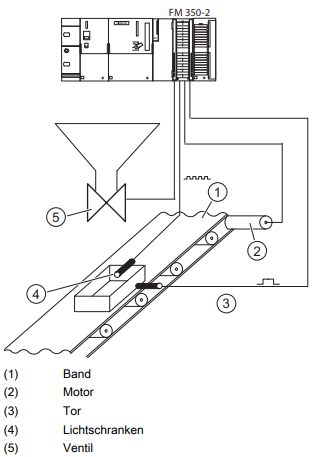
\includegraphics[width=0.8\textwidth]{Fotos/Beispiel_fm350-2.png}
    \caption{Beispiel für den Einsatz einer FM 350-2 in der S7-300 \cite{fm350_Handbuch}}
    \label{fig:fm350-2}
\end{figure}



%//////////////////////////////////////////////////////////////////////////////////////////////////////////////////////
%//////////////////////////////////////////////////////////////////////////////////////////////////////////////////////
\section{Vorteile und neue Möglichkeiten durch das TM FAST Modul} 

%//////////////////////////////////////////////////////////////////////////////////////////////////////////////////////
%//////////////////////////////////////////////////////////////////////////////////////////////////////////////////////
\section{Anforderungen an die Neuentwicklung} 


\begin{table}[h]
    \centering
    \renewcommand{\arraystretch}{1.3}
    \begin{tabularx}{\textwidth}{|X|X|X|}
        \hline
        \textbf{Kriterium} & \textbf{TM FAST} & \textbf{FM 350-2} \\
        \hline
        \multicolumn{3}{|c|}{\textbf{Unterschiede}} \\
        \hline
        Architektur & FPGA-basiert, flexible und programmierbare Hardwareplattform & Reines Zählermodul ohne FPGA-Technologie \\
        \hline
        Funktionalität & Kann komplexe Prozesssteuerungs- und Überwachungsaufgaben übernehmen & Spezialisiert auf Zählen, Frequenz- und Drehzahlmessung \\
        \hline
        Prozessintegration & Kann direkt in den Produktionsprozess eingreifen und Prozessalarme auslösen & Liefert Zähler- und Messwerte, die von der übergeordneten Steuerung weiterverarbeitet werden \\
        \hline
        Flexibilität & Hohe Flexibilität und Anpassungsfähigkeit durch FPGA-Architektur & Festgelegte Funktionalität, die nicht ohne Weiteres erweitert werden kann \\
        \hline
        \multicolumn{3}{|c|}{\textbf{Gemeinsamkeiten}} \\
        \hline
        Zählfunktionen & \multicolumn{2}{c|}{Beide Module bieten Zählfunktionen mit hoher Auflösung (z.B. 32-Bit Zähltiefe)} \\
        \hline
        Frequenz- und Drehzahlmessung & \multicolumn{2}{c|}{Beide Module unterstützen die Messung von Frequenzen und Drehzahlen} \\
        \hline
        Einbindung in Steuerungsarchitektur & \multicolumn{2}{c|}{Beide Module werden in die übergeordnete Steuerungsarchitektur integriert} \\
        \hline
        Industrielle Anwendungen & \multicolumn{2}{c|}{Beide Module finden Einsatz in ähnlichen Industriebereichen wie Verpackung, Sortierung, Dosierung etc.} \\
        \hline
    \end{tabularx}
    \caption{Vergleich zwischen TM FAST und FM 350-2}
    \label{tab:tm_fast_vs_fm350-2}
\end{table}

% \begin{table}[h]     funktioniert
%     \centering
%     \renewcommand{\arraystretch}{1.3} % Erhöht den Zeilenabstand leicht
%     \begin{tabularx}{\textwidth}{|X|X|X|}
%         \hline
%         \textbf{Kriterium} & \textbf{TM FAST} & \textbf{FM 350-2} \\\multicolumn{3}{|c|}{\textbf{Unterschiede}} \\
%         \hline
%         Architektur & FPGA-basiert, flexible und programmierbare Hardwareplattform & Reines Zählermodul ohne FPGA-Technologie \\
%         \hline
%         Funktionalität & Kann komplexe Prozesssteuerungs- und Überwachungsaufgaben übernehmen & Spezialisiert auf Zählen, Frequenz- und Drehzahlmessung \\
%         \hline
%         Prozessintegration & Kann direkt in den Produktionsprozess eingreifen und Prozessalarme auslösen & Liefert Zähler- und Messwerte, die von der übergeordneten Steuerung weiterverarbeitet werden \\
%         \hline
%         Flexibilität & Hohe Flexibilität und Anpassungsfähigkeit durch FPGA-Architektur & Festgelegte Funktionalität, die nicht ohne Weiteres erweitert werden kann \\
%         \hline
%     \end{tabularx}
%     \caption{Vergleich zwischen TM FAST und FM 350-2}
%     \label{tab:tm_fast_vs_fm350-2}
% \end{table}











\newif\ifdraft
%\drafttrue 
\draftfalse
\ifdraft

\chapter{Analyse der Ablösung des FM350-2 durch das TM FAST Modul}

\section{Funktionsweise und Limitierungen des FM350-2} 
\section{Vorteile und neue Möglichkeiten durch das TM FAST Modul} 
\section{Anforderungen an die Neuentwicklung} 



Unterschiede in der Aufgabe und Softwarearchetektur:

\begin{table}[h]
    \centering
    \renewcommand{\arraystretch}{1.3}
    \begin{tabularx}{\textwidth}{|X|X|X|}
        \hline
        \textbf{Kriterium} & \textbf{TM FAST} & \textbf{FM 350-2} \\
        \hline
        \multicolumn{3}{|c|}{\textbf{Unterschiede}} \\
        \hline
        Architektur & FPGA-basiert, flexible und programmierbare Hardwareplattform & Reines Zählermodul ohne FPGA-Technologie \\
        \hline
        Funktionalität & Kann komplexe Prozesssteuerungs- und Überwachungsaufgaben übernehmen & Spezialisiert auf Zählen, Frequenz- und Drehzahlmessung \\
        \hline
        Prozessintegration & Kann direkt in den Produktionsprozess eingreifen und Prozessalarme auslösen & Liefert Zähler- und Messwerte, die von der übergeordneten Steuerung weiterverarbeitet werden \\
        \hline
        Flexibilität & Hohe Flexibilität und Anpassungsfähigkeit durch FPGA-Architektur & Festgelegte Funktionalität, die nicht ohne Weiteres erweitert werden kann \\
        \hline
        \multicolumn{3}{|c|}{\textbf{Gemeinsamkeiten}} \\
        \hline
        Zählfunktionen & \multicolumn{2}{c|}{Beide Module bieten Zählfunktionen mit hoher Auflösung (z.B. 32-Bit Zähltiefe)} \\
        \hline
        Frequenz- und Drehzahlmessung & \multicolumn{2}{c|}{Beide Module unterstützen die Messung von Frequenzen und Drehzahlen} \\
        \hline
        Einbindung in Steuerungsarchitektur & \multicolumn{2}{c|}{Beide Module werden in die übergeordnete Steuerungsarchitektur integriert} \\
        \hline
        Industrielle Anwendungen & \multicolumn{2}{c|}{Beide Module finden Einsatz in ähnlichen Industriebereichen wie Verpackung, Sortierung, Dosierung etc.} \\
        \hline
    \end{tabularx}
    \caption{Vergleich zwischen TM FAST und FM 350-2}
    \label{tab:tm_fast_vs_fm350-2}
\end{table}

% \begin{table}[h]     funktioniert
%     \centering
%     \renewcommand{\arraystretch}{1.3} % Erhöht den Zeilenabstand leicht
%     \begin{tabularx}{\textwidth}{|X|X|X|}
%         \hline
%         \textbf{Kriterium} & \textbf{TM FAST} & \textbf{FM 350-2} \\\multicolumn{3}{|c|}{\textbf{Unterschiede}} \\
%         \hline
%         Architektur & FPGA-basiert, flexible und programmierbare Hardwareplattform & Reines Zählermodul ohne FPGA-Technologie \\
%         \hline
%         Funktionalität & Kann komplexe Prozesssteuerungs- und Überwachungsaufgaben übernehmen & Spezialisiert auf Zählen, Frequenz- und Drehzahlmessung \\
%         \hline
%         Prozessintegration & Kann direkt in den Produktionsprozess eingreifen und Prozessalarme auslösen & Liefert Zähler- und Messwerte, die von der übergeordneten Steuerung weiterverarbeitet werden \\
%         \hline
%         Flexibilität & Hohe Flexibilität und Anpassungsfähigkeit durch FPGA-Architektur & Festgelegte Funktionalität, die nicht ohne Weiteres erweitert werden kann \\
%         \hline
%     \end{tabularx}
%     \caption{Vergleich zwischen TM FAST und FM 350-2}
%     \label{tab:tm_fast_vs_fm350-2}
% \end{table}

\section{Funktionalität und Schnittstellen des FM350-2-Moduls}

\subsection{Funktionen}

\subsubsection{Die Funktion \texttt{FC CNT2\_CTR} (FC2), Baugruppe steuern}

\begin{itemize}
    \item \textbf{Aufgabe: } Mit der \texttt{FC CNT2\_CTR} steuern Sie die Digitalausgänge (Freigabe und Sperrung) sowie die Software-Tore der FM 350-2. Außerdem erhalten Sie Rückmeldungen von der FM 350-2.
    \item \textbf{Aktion: } Die \texttt{FC CNT2\_CTR} führt folgende Aktionen durch: 
                            \subitem 1. Zähler-DB initialisieren 
                            \subitem 2. Lesen der Rückmeldesignale. Die gelesenen Werte werden vom FC im Zähler-DB in der 
                            Struktur CHECKBACK\_SIGNALS abgelegt. 
                            \subitem 3. Übertragen der Steuersignale aus dem Zähler-DB (Struktur CONTROL\_SIGNALS) zur 
                            FM 350-2.
    \item \textbf{Aufruf: } Sie müssen die \texttt{FC CNT2\_CTR} zyklisch (im OB1 oder in den Weckalarmen - nur OB35 in 
    S7-300) für jede Baugruppe aufrufen. Der Aufruf in einem Alarmprogramm ist nicht zulässig. 
    Vor dem Aufruf der \texttt{FC CNT2\_CTR} tragen Sie die aktuellen Steuersignale in der Struktur 
    CONTROL\_SIGNALS im Zähler-DB ein. Nach dem Aufruf der \texttt{FC CNT2\_CTR} sind die 
    Rückmeldesignale in der Struktur CHECKBACK\_SIGNALS im Zähler-DB aktualisiert und Sie 
    können diese von dort weiterverarbeiten. 
    Die Nummer des Zähler-DBs wird beim Aufruf des FC an dem Parameter DB\_NO 
    angegeben.
\end{itemize}

\subsubsection{Zählerstände, Grenzwerte und Vergleichswerte laden (\texttt{FC3} / \texttt{FB3})}

Mit der \texttt{FC CNT2\_WR} / \texttt{FB CNT2WRPN} laden Sie die Zähler und Vergleicher der FM 350-2 
mittels Schreibaufträgen. Dazu müssen Sie die \texttt{FC CNT2\_WR} / \texttt{FB CNT2WRPN} bei Bedarf 
pro Baugruppe aufrufen.  
Sie binden die Funktion \texttt{FC CNT2\_WR} / \texttt{FB CNT2WRPN} nur in Ihr Programm ein, wenn Sie 
die Zähler und Vergleicher der FM 350-2 im Betrieb neu laden müssen.
 
\subsection{Zähl- und Messwerte auslesen (\texttt{FC4} / \texttt{FB4})}

Mit der \texttt{FC CNT2\_RD} / \texttt{FB CNT2RDPN} lesen Sie Zähl- und Messwerte von der FM 350-2 
mit Leseaufträgen. Dazu rufen Sie die \texttt{FC CNT2\_RD} / \texttt{FB CNT2RDPN} zyklisch einmal pro 
Baugruppe auf.  
Sie binden die \texttt{FC CNT2\_RD} / \texttt{FB CNT2RDPN} nicht in Ihr Anwenderprogramm ein, wenn 
Sie keine Leseaufträge bearbeiten.

\subsection{Die Funktion \texttt{FC DIAG\_RD} (FC5), Diagnosedaten lesen}

Mit der \texttt{FC DIAG\_RD} können Sie im Falle eines Diagnosealarms die Diagnosealarmdaten in 
den Zähler-DB laden.


\section{Einsatzgebiete der FM 350-2 / evtl nicht nötig}

\subsection{Haupteinsatzgebiet} Das Haupteinsatzgebiet der FM 350-2 liegt dort, wo Signale gezählt und schnelle Reaktionen auf einen vorgegebenen Zählerstand ausgelöst werden müssen sowie Frequenzen oder Drehzahlen gemessen werden sollen.

\subsection{Beispiele für den Einsatz} Beispiele hierfür sind: \begin{itemize} \item Verpackungsanlagen \item Sortieranlagen \item Dosieranlagen \item Drehzahlregelungen und Überwachung von Gasturbinen \end{itemize}

\subsection{Beispiel für den Einsatz einer FM 350-2} Aus einem Sammelbehälter soll eine bestimmte Anzahl Teile in einen Karton abgefüllt werden. Der Zählkanal 0 zählt die Teile und steuert das Ventil zur Abfüllung. Mit dem Zählkanal 1 wird der Motor zum Transport der Kartons gesteuert und die Anzahl der Kartons gezählt.

Befindet sich der Karton in der richtigen Position wird das Ventil geöffnet und die Teile werden abgefüllt. Ist die vorgegebene Anzahl erreicht, wird das Ventil geschlossen und der Transport des Kartons angestoßen. Nachfallende Teile werden mitgezählt bis ein neuer Karton eintrifft.
Während des Transports der Kartons ist eine neue Anzahl Teile vorgebbar. Die abgefüllten Teile sowie die Anzahl der Kartons ist beobachtbar. 
\fi
\chapter{Entwicklung des VHDL-basierten Applikationsbeispiels}

\section{Konzept und Architektur des neuen Applikationsdesigns}

Byte Zuweisung für FB\_IF (32 Byte)
    \begin{itemize}
        \item 3 Byte für Kanalobergrenze = 4095 (Standartventil ist 1 Impuls/ 1 ml -> 4l abfüllung) => bis zu 10 Kanäle möglich
        \item 4 Byte für Kanalobergrenze = 65535 (65l abfüllung) => nur 8 Kanäle möglich
    \end{itemize}

Andere Ideen:
Vieleicht auf TMFASTUserWriteREC ausweichen? (Bis zu 128 Byte)
asynchron ( was ist wenn daten mitten im ablauf geändert werden?)

Algorithmus, der im ersten Zyklus die Kanalobergrenzen 1–4 von der CPU an das TMFast sendet, im zweiten Zyklus 5–8 usw.
ist synchron und eignet sich besser
die Steuerschnittstelle, da über die im Betrieb auch taktsynchron neue Werte geschrieben werden können. Der Nachteil des Write-Records ist die Asynchronität zum Zyklus.


Zähler -> Unter- und Obergrenze einstellbar

CPU Stop beachten:
% /*if CPU_STOP = '1' then
% 					STATUS_DQ  <= ( others => '0' );
% 					STATUS_TX  <= ( others => '0' );
% 				end if;*/

Questa DQ fehler beheben /evtl Hello world datei probieren um fehler zu finden
\section{Umsetzung der Funktionalität in VHDL}
\section{Test und Validierung der VHDL-Implementierung}
\section{Vergleich mit der bisherigen Lösung}
\chapter{Integration in das TIA Portal?} %fleißarbeit -> außer es ist herausforderung
\section{Herausforderungen der Einbindung des TM FAST Moduls}
\section{Anpassungen an die Projektumgebung}
\section{Implementierung und Tests im TIA Portal}
\section{Evaluation der neuen Lösung im industriellen Kontext}
\chapter{Aspekte des Software Engineerings} %gehört in andere kapitel, aber nicht in die Bachelorarbeit -> KANN ALSO RAUS (ehr ins 4.Kapitel)
\section{Best Practices in der VHDL-Entwicklung}
\section{Modularisierung und Wiederverwendbarkeit}
\section{Teststrategien und Debugging-Techniken}
\section{Dokumentation und Wartung der Software}
\chapter{Fazit und Ausblick}
\section{Zusammenfassung der Ergebnisse}
\section{Kritische Reflexion und Herausforderungen}
\section{Potenzielle Weiterentwicklungen und zukünftige Anwendungen}
%\include{content/9_Ende}
%\chapter{Analyse}

Unterschiede in der Aufgabe und Softwarearchetektur:

\begin{table}[h]
    \centering
    \renewcommand{\arraystretch}{1.3}
    \begin{tabularx}{\textwidth}{|X|X|X|}
        \hline
        \textbf{Kriterium} & \textbf{TM FAST} & \textbf{FM 350-2} \\
        \hline
        \multicolumn{3}{|c|}{\textbf{Unterschiede}} \\
        \hline
        Architektur & FPGA-basiert, flexible und programmierbare Hardwareplattform & Reines Zählermodul ohne FPGA-Technologie \\
        \hline
        Funktionalität & Kann komplexe Prozesssteuerungs- und Überwachungsaufgaben übernehmen & Spezialisiert auf Zählen, Frequenz- und Drehzahlmessung \\
        \hline
        Prozessintegration & Kann direkt in den Produktionsprozess eingreifen und Prozessalarme auslösen & Liefert Zähler- und Messwerte, die von der übergeordneten Steuerung weiterverarbeitet werden \\
        \hline
        Flexibilität & Hohe Flexibilität und Anpassungsfähigkeit durch FPGA-Architektur & Festgelegte Funktionalität, die nicht ohne Weiteres erweitert werden kann \\
        \hline
        \multicolumn{3}{|c|}{\textbf{Gemeinsamkeiten}} \\
        \hline
        Zählfunktionen & \multicolumn{2}{c|}{Beide Module bieten Zählfunktionen mit hoher Auflösung (z.B. 32-Bit Zähltiefe)} \\
        \hline
        Frequenz- und Drehzahlmessung & \multicolumn{2}{c|}{Beide Module unterstützen die Messung von Frequenzen und Drehzahlen} \\
        \hline
        Einbindung in Steuerungsarchitektur & \multicolumn{2}{c|}{Beide Module werden in die übergeordnete Steuerungsarchitektur integriert} \\
        \hline
        Industrielle Anwendungen & \multicolumn{2}{c|}{Beide Module finden Einsatz in ähnlichen Industriebereichen wie Verpackung, Sortierung, Dosierung etc.} \\
        \hline
    \end{tabularx}
    \caption{Vergleich zwischen TM FAST und FM 350-2}
    \label{tab:tm_fast_vs_fm350-2}
\end{table}

% \begin{table}[h]     funktioniert
%     \centering
%     \renewcommand{\arraystretch}{1.3} % Erhöht den Zeilenabstand leicht
%     \begin{tabularx}{\textwidth}{|X|X|X|}
%         \hline
%         \textbf{Kriterium} & \textbf{TM FAST} & \textbf{FM 350-2} \\\multicolumn{3}{|c|}{\textbf{Unterschiede}} \\
%         \hline
%         Architektur & FPGA-basiert, flexible und programmierbare Hardwareplattform & Reines Zählermodul ohne FPGA-Technologie \\
%         \hline
%         Funktionalität & Kann komplexe Prozesssteuerungs- und Überwachungsaufgaben übernehmen & Spezialisiert auf Zählen, Frequenz- und Drehzahlmessung \\
%         \hline
%         Prozessintegration & Kann direkt in den Produktionsprozess eingreifen und Prozessalarme auslösen & Liefert Zähler- und Messwerte, die von der übergeordneten Steuerung weiterverarbeitet werden \\
%         \hline
%         Flexibilität & Hohe Flexibilität und Anpassungsfähigkeit durch FPGA-Architektur & Festgelegte Funktionalität, die nicht ohne Weiteres erweitert werden kann \\
%         \hline
%     \end{tabularx}
%     \caption{Vergleich zwischen TM FAST und FM 350-2}
%     \label{tab:tm_fast_vs_fm350-2}
% \end{table}

\section{Funktionalität und Schnittstellen des FM350-2-Moduls}

\subsection{Funktionen}

\subsubsection{Die Funktion \texttt{FC CNT2\_CTR} (FC2), Baugruppe steuern}

\begin{itemize}
    \item \textbf{Aufgabe: } Mit der \texttt{FC CNT2\_CTR} steuern Sie die Digitalausgänge (Freigabe und Sperrung) sowie die Software-Tore der FM 350-2. Außerdem erhalten Sie Rückmeldungen von der FM 350-2.
    \item \textbf{Aktion: } Die \texttt{FC CNT2\_CTR} führt folgende Aktionen durch: 
                            \subitem 1. Zähler-DB initialisieren 
                            \subitem 2. Lesen der Rückmeldesignale. Die gelesenen Werte werden vom FC im Zähler-DB in der 
                            Struktur CHECKBACK\_SIGNALS abgelegt. 
                            \subitem 3. Übertragen der Steuersignale aus dem Zähler-DB (Struktur CONTROL\_SIGNALS) zur 
                            FM 350-2.
    \item \textbf{Aufruf: } Sie müssen die \texttt{FC CNT2\_CTR} zyklisch (im OB1 oder in den Weckalarmen - nur OB35 in 
    S7-300) für jede Baugruppe aufrufen. Der Aufruf in einem Alarmprogramm ist nicht zulässig. 
    Vor dem Aufruf der \texttt{FC CNT2\_CTR} tragen Sie die aktuellen Steuersignale in der Struktur 
    CONTROL\_SIGNALS im Zähler-DB ein. Nach dem Aufruf der \texttt{FC CNT2\_CTR} sind die 
    Rückmeldesignale in der Struktur CHECKBACK\_SIGNALS im Zähler-DB aktualisiert und Sie 
    können diese von dort weiterverarbeiten. 
    Die Nummer des Zähler-DBs wird beim Aufruf des FC an dem Parameter DB\_NO 
    angegeben.
\end{itemize}

\subsubsection{Zählerstände, Grenzwerte und Vergleichswerte laden (\texttt{FC3} / \texttt{FB3})}

Mit der \texttt{FC CNT2\_WR} / \texttt{FB CNT2WRPN} laden Sie die Zähler und Vergleicher der FM 350-2 
mittels Schreibaufträgen. Dazu müssen Sie die \texttt{FC CNT2\_WR} / \texttt{FB CNT2WRPN} bei Bedarf 
pro Baugruppe aufrufen.  
Sie binden die Funktion \texttt{FC CNT2\_WR} / \texttt{FB CNT2WRPN} nur in Ihr Programm ein, wenn Sie 
die Zähler und Vergleicher der FM 350-2 im Betrieb neu laden müssen.
 
\subsection{Zähl- und Messwerte auslesen (\texttt{FC4} / \texttt{FB4})}

Mit der \texttt{FC CNT2\_RD} / \texttt{FB CNT2RDPN} lesen Sie Zähl- und Messwerte von der FM 350-2 
mit Leseaufträgen. Dazu rufen Sie die \texttt{FC CNT2\_RD} / \texttt{FB CNT2RDPN} zyklisch einmal pro 
Baugruppe auf.  
Sie binden die \texttt{FC CNT2\_RD} / \texttt{FB CNT2RDPN} nicht in Ihr Anwenderprogramm ein, wenn 
Sie keine Leseaufträge bearbeiten.

\subsection{Die Funktion \texttt{FC DIAG\_RD} (FC5), Diagnosedaten lesen}

Mit der \texttt{FC DIAG\_RD} können Sie im Falle eines Diagnosealarms die Diagnosealarmdaten in 
den Zähler-DB laden.


\section{Einsatzgebiete der FM 350-2}

\subsection{Haupteinsatzgebiet} Das Haupteinsatzgebiet der FM 350-2 liegt dort, wo Signale gezählt und schnelle Reaktionen auf einen vorgegebenen Zählerstand ausgelöst werden müssen sowie Frequenzen oder Drehzahlen gemessen werden sollen.

\subsection{Beispiele für den Einsatz} Beispiele hierfür sind: \begin{itemize} \item Verpackungsanlagen \item Sortieranlagen \item Dosieranlagen \item Drehzahlregelungen und Überwachung von Gasturbinen \end{itemize}

\subsection{Beispiel für den Einsatz einer FM 350-2} Aus einem Sammelbehälter soll eine bestimmte Anzahl Teile in einen Karton abgefüllt werden. Der Zählkanal 0 zählt die Teile und steuert das Ventil zur Abfüllung. Mit dem Zählkanal 1 wird der Motor zum Transport der Kartons gesteuert und die Anzahl der Kartons gezählt.

Befindet sich der Karton in der richtigen Position wird das Ventil geöffnet und die Teile werden abgefüllt. Ist die vorgegebene Anzahl erreicht, wird das Ventil geschlossen und der Transport des Kartons angestoßen. Nachfallende Teile werden mitgezählt bis ein neuer Karton eintrifft.
Während des Transports der Kartons ist eine neue Anzahl Teile vorgebbar. Die abgefüllten Teile sowie die Anzahl der Kartons ist beobachtbar. 

\begin{figure}[h!] % "H" zwingt die Position der Abbildung genau hier \centering
    \includegraphics[width=0.8\textwidth]{Fotos/Beispiel für den Einsatz einer FM 350-2 in der S7-300.png} 
    \caption{Beispiel für den Einsatz einer FM 350-2 in der S7-300\cite{fm350_Handbuch}} 
    \label{fig:Beispiel für den Einsatz einer FM 350-2 in der S7-300} % Für spätere Verweise im Text. 
    \vspace{0.5em} % Optional: Abstand zwischen Bildunterschrift und Zusatztext 
    \small % Schriftgröße anpassen, falls gewünscht 
\end{figure}
\bibliographystyle{plain}   % Wähle einen Zitierstil (z. B. plain, alpha, IEEE)

\begin{thebibliography}{}

\bibitem{klett2004}
Ernst Klett Verlag (2004): \textit{Infoblatt Siemens AG}. Verfügbar unter: \url{https://www.klett.de/alias/1036900}. Zugriff: 5. Januar 2025.

\bibitem{merkur2022}
Merkur (2022): \textit{Siemens – Geschichte, Aktie und Tätigkeitsfelder}. Verfügbar unter: \url{https://www.merkur.de/wirtschaft/siemens-geschichte-aktie-und-taetigkeitsfelder-91268844.html}. Zugriff: 19. Januar 2024.

\bibitem{statista2025}
Siemens, 2023, zitiert nach de.statista.com: \textit{Umsatz von Siemens SE seit 2005}. Verfügbar unter: \url{https://de-statista-com.thn.idm.oclc.org/statistik/daten/studie/73827/umfrage/umsatz-von-siemens-seit-2005/}. Zugriff: 5. Januar 2025.

\bibitem{researchgate}
ResearchGate: Verfügbar unter: \url{https://www.researchgate.net/figure/SA-88s-physical-model-and-an-example-production-allocation_fig2_308384237/}. Zugriff: 11. Januar 2025.

\bibitem{siemens2022}
Siemens (2022): \textit{Pflichtenheft-SmartFactory}. Internes Dokument.

\bibitem{bee2022}
Liam Bee (2022): \textit{PLC and HMI development with Siemens TIA Portal: develop PLC and HMI programs using standard methods and structured approaches with TIA Portal V17}. Packt Publishing, Limited. 


%---------------------------------------------------------------------------------------------


\bibitem{fm350_Handbuch}
Siemens AG (2011): \textit{Zählerbaugruppe FM 350-2 Gerätehandbuch}. Verfügbar unter: \url{https://cache.industry.siemens.com/dl/files/178/1105178/att_20226/v1/s7300_fm350_2_operating_instructions_de_de-DE.pdf}. Zugriff 11. März 2025.

\bibitem{TmFast_progrmming_manual}
Siemens AG (2023): \textit{TMFast Programmeier Handbuch}. Verfügbar unter: \url{https://cache.industry.siemens.com/dl/files/088/109816088/att_1144842/v2/s71500_tm_fast_programming_manual_de-DE_de-DE.pdf}. Zugriff 12. März 2025.


\end{thebibliography}
\chapter{Plan} 

Hier sind einige Schritte, die Ihnen dabei helfen können, eine VHDL-Applikation für das TM FAST-Modul zu entwickeln, um das alte 
FM350-2-Modul zu ersetzen:

\subsection*{Anforderungsanalyse} 
\begin{itemize} 
    \item Analysieren Sie sorgfältig die Funktionalität und Schnittstellen des FM350-2-Moduls. 
    \item Identifizieren Sie die Kernfunktionen, die das neue TM FAST-Modul erfüllen muss. 
    \item Definieren Sie klar die Eingangs- und Ausgangssignale, die Kommunikationsprotokolle und andere relevante Spezifikationen. 
\end{itemize}

\subsection*{Architekturentwurf} 
\begin{itemize} 
    \item Entwerfen Sie eine modulare Architektur für Ihre VHDL-Applikation. 
    \item Unterteilen Sie die Funktionalität in logische Blöcke wie Steuerungslogik, Kommunikationsschnittstellen, Datenpfade usw. 
    \item Legen Sie die Schnittstellen zwischen den einzelnen Modulen fest. 
\end{itemize}

\subsection*{VHDL-Entwicklung} 
\begin{itemize} 
    \item Beginnen Sie mit der Implementierung der einzelnen VHDL-Module basierend auf Ihrem Architekturentwurf. 
    \item Achten Sie auf eine strukturierte und modulare Codeerstellung, um die Wartbarkeit und Erweiterbarkeit zu erleichtern. 
    \item Verwenden Sie VHDL-Sprachkonstrukte wie Prozesse, Signale, Typen und Pakete, um Ihre Applikation übersichtlich und 
    effizient zu gestalten. 
\end{itemize}

\subsection*{Simulation und Test} 
\begin{itemize} 
    \item Erstellen Sie umfangreiche Testbänke, um Ihre VHDL-Applikation gründlich zu überprüfen. 
    \item Führen Sie Simulationen durch, um das korrekte Verhalten der einzelnen Module und der Gesamtapplikation zu verifizieren. 
    \item Testen Sie die Applikation schrittweise, um mögliche Fehler frühzeitig zu erkennen und zu beheben. 
\end{itemize}

\subsection*{Integration und Validierung} 
\begin{itemize} 
    \item Integrieren Sie Ihre VHDL-Applikation in die Gesamtarchitektur des TM FAST-Moduls. 
    \item Testen Sie die Applikation in der realen Umgebung, um ihre Kompatibilität und Funktionalität zu validieren. 
    \item Passen Sie die Applikation gegebenenfalls an, um Anforderungen und Spezifikationen des TM FAST-Moduls zu erfüllen. 
\end{itemize}

\subsection*{Dokumentation und Versionskontrolle} 
\begin{itemize} 
    \item Erstellen Sie eine ausführliche Dokumentation, die die Architektur, Schnittstellen, Konfiguration und Verwendung Ihrer 
    VHDL-Applikation beschreibt. 
    \item Nutzen Sie ein geeignetes Versionskontrollsystem, um Änderungen an Ihrer Applikation nachzuverfolgen und zu verwalten. 
\end{itemize}

Durch diese strukturierte Vorgehensweise können Sie sicherstellen, dass Ihre VHDL-Applikation für das TM FAST-Modul die 
Anforderungen des FM350-2-Moduls erfüllt und in die Gesamtarchitektur des TM FAST-Systems nahtlos integriert wird.

\chapter{Fragen}
Müssen Alarme umgesetzt werden? ->Müssen nicht berücksichtigt werden
Müssen Hardwareconfigs von der CPU oder von TMFast gehandhabt werden? ->hardwareconfig der (z.B. Ventile) ist in VHDL (andere Kommunikationsprotokole und co pro z.B. Ventile)
Wie verhalten sich die In- und Outputs? 
\begin{itemize}
    \item Sollen alle Eingänge Zähl- und Richtungseingang sein oder Aufteilung zwischen den beiden? Nur zähler
    \item 
\end{itemize}

wie funktionieren ventile überhaupt?

bit an die cpu senden 

nachlauf bei inkrement zum abfüllen

cpu macht  - tm fast macht ventil zu

auf ist 1 zu ist low für ventil

abfüllende menge muss übergeben werden

vhdl auf hoher ebene darstellen (als baustein)

syncron oder asyncron (für zähler oder generell) -> Alles Syncron (TM Fast arbeitet (einstellbar mit 50mHz) schneller als ein ventil) -> dadurch zählt es schneller als ikremente des ventils

clk wird bei änderung aktiviert (High->Low / Low->High)

steuerung des ventils über PLC oder TMFAST? Erstamal Plc mit bool senden (überlauf für counter (justierung)) / TMFast erfordert Kommunikations-Protokolle

Filter?

Anwendung in mehreren oder einem Process in vhdl?

soll der timer nur zählen, wenn die flanke positiv wird? oder auch wenn sie negativ wird? -> nur bei positiv

Allgemein:
Schriftgröße und Seitenränder?
Zitieren von Handbüchern (Graue Literatur) und ChatGPT?

\chapter{Tests}

rückgabe über das (fb\_if) feedback\_interface

EncEmu encoder für impulse 

schwierigkeit: di1 oder di0 zählen

RD\_Rec sind azyklisch und nur selten benutzt

library test 8 counter -> name mit test cases Jürgen, ..., Kollege aus Prag

Muss ich nicht allein schreiben

Mathias fragen wenn funktionierendes Programm -> in den Nightly test muss in den nightly build

-systemlogic updaten auf v2 

-zähler des sea teams verwenden

- 0000\_0000\_0000\_0000\_0000\_0000\_0000\_0001 -> FB\_IF(0)(0)<='1';
-    /->Q0.0                          (FB\_IF(0))

- FB\_IF(1)(0) == QD4
\chapter{Passwörter}

PLC: Siemens123

\backmatter

\end{document}
